\chapter{Построение конвейера машинного обучения. Генерация данных} \label{ch2}

Данная глава посвящена исследованиям, проведённым для построения конвейера машинного обучения. В параграфе \ref{ch2:sec1} приведено описание object detection задачи машинного обучения и выбранной для этого модели. В параграфе \ref{ch2:sec2} описан первоначальный конвейер моделей, с помощью которого предполагалось решать задачу. Описан процесс генерации данных для используемой object detection модели, результаты обучения модели. В параграфе \ref{ch2:sec3} предложены исправления, необходимые для повышения качества обучения модели и  показаны результаты обучения object detection модели на итоговом варианте. Далее, приводится методика генерации данных для обучения вспомогательных сетей, решение об использовании которых было принято по результатам проведённых ранее экспериментов. Показаны результаты обучения вспомогательных моделей.

\section{Object detection задача. Модель Detectron2 Faster R-CNN} \label{ch2:sec1}

Object detection задача состоит в необходимости найти область интереса -- region of interest, ROI в виде баундбокса, то есть прямоугольника, стороны которого параллельны сторонам экрана, и который содержит объект интереса.

Для выполнения данной работы была использована модель Detectron2 Faster R-CNN ResNet 50 FPN \cite{detectron}.

\subsection{Архитектура Detectron2 Faster R-CNN ResNet 50 FPN}

Для того, чтобы детально описать архитектуру сети Detectron2 Faster R-CNN, необходимо сначала описать архитектуру сетей предыдущего поколения R-CNN и Fast R-CNN.

\subsubsection{Архитектура R-CNN}

\textbf{R-CNN}, основоположник модели Faster R-CNN -- одна из первых моделей, применённых для обнаружения объекта на картинке \cite{rcnn}.

Его архитектура состоит из следующих шагов:

\begin{enumerate}[1.]
	\item Определение набора гипотез.
	\item Извлечение из предполагаемых регионов признаков с помощью сверточной нейронной сети и их кодирование в вектор.
	\item Классификация объекта внутри гипотезы на основе вектора из шага 2.
	\item Улучшение (корректировка) координат гипотезы.
	\item Повтор шагов 2-4, пока не будут обработаны все гипотезы.
\end{enumerate}

Опишем каждый этап подробнее.

\begin{itemize}
	\item \textbf{Поиск гипотез}. Изображение на входе первым делом разбивается на маленькие гипотезы разных размеров. Для этого используется алгоритм Selective Search \cite{ssearch}. Таким образом выделяется примерно 2000 разных регионов, которые частично друг друга перекрывают. Для более точной последующей обработки каждая гипотеза дополнительно расширяется на 16 пикселей во всех 4 направлениях -- как бы добавляя \textit{контекст}.
	
	\item \textbf{Кодирование признаков в вектор}. Каждая гипотеза из предыдущего шага независимо и по отдельности друг от друга поступает на вход сверточной нейронной сети. В качестве нее используется архитектура AlexNet без последнего softmax-слоя. Главной задачей сети является кодирование поступаемого изображения в векторное представление, которое извлекается из последнего полносвязного FC7 слоя. Так на выходе получается 4096-размерное векторное представление.
	
	\item \textbf{Классификация}. После получения характеризующего гипотезу вектора становится возможна ее дальнейшая обработка. Для определения, какой именно объект находится в предполагаемом регионе, авторы используют классический метод классификации разделяющими плоскостями на базе SVM. SVM работает по принципу OvR: One vs. Rest -- один против всех, один из методов мультиклассовой классификации. Таким образом, фактически решается задача бинарной классификации -- есть ли конкретный класс объекта внутри предполагаемого региона или нет. Таким образом, выходом является размерный вектор, отображающий уверенность в конкретном классе содержащегося в гипотезе объекта.
	
	\item \textbf{Уточнение гипотез}. 
	Гипотезы, полученные на шаге 1, не всегда содержат правильные координаты, например, объект может быть неудачно <<обрезан>>. Поэтому необходимо их дальнейшее уточнение. Так, гипотезы, содержащие какой-либо объект (наличие объекта определяется на шаге классификации), дополнительно обрабатываются линейной регрессией. То есть гипотезы с классом «фон» не нуждаются в дополнительной обработке регионов, ведь на самом деле там нет объекта.
	
	Каждый объект, специфично для своего класса, имеет определенные размеры и соотношения сторон, поэтому рекомендуется применять собственный регрессор на каждый класс.
	
	В отличие от предыдущего шага, авторы для наилучшей работы используют на входе не вектор из слоя FC7, а карты признаков, извлеченные из последнего MaxPooling слоя (в AlexNet его размерность составляет 256×6×6). Это объясняется тем, что  вектор сохраняет информацию о наличии объекта с какими-то характеристическими подробностями, а карта признаков наилучшим образом сохраняет информацию о местоположении объектов.
	
\end{itemize}

\subsubsection{Архитектура Fast R-CNN}

Данная архитектура является улучшенным вариантом архитектуры R-CNN. Целью её создания было, в первую очередь, ускорение процесса обучения и инференса. Рассмотрим этапы, через которые проходит изображение при обработке Fast R-CNN \cite{fasterrcnn}.

\begin{itemize}
	\item Извлечение карты признаков изображения (не для каждой гипотезы по отдельности, а для всего изображения целиком)
	\item Поиск гипотез -- остался без изменения
	\item Сопоставление каждой гипотезы с местом на карте признаков, то есть использование единого набора выделенных признаков для каждой гипотезы (координаты гипотез можно однозначно сопоставить с местоположением на карте признаков)
	\item Классификация каждой гипотезы и исправление координат ограничивающей рамки (эту часть стало возможным запускать параллельно, поскольку больше нет зависимости от SVM-классификации)
\end{itemize}

В изначальной концепции R-CNN каждая предложенная гипотеза по отдельности обрабатывается с помощью CNN -- этот этап стал бутылочным горлышком для всей архитектуры. Для решения этой проблемы был разработан Region of Interest (RoI) слой. Этот слой позволяет единожды обрабатывать изображение целиком с помощью нейронной сети, получая на выходе карту признаков, которая далее используется для обработки каждой гипотезы.

Основной задачей RoI слоя является сопоставление координат гипотез (координаты баундбоксов) соответствующим координатам карты признаков. Делая <<срез>> карты признаков, RoI слой подает его на вход полносвязному слою для последующего определения класса и поправок к координатам (см. следующие разделы).

В R-CNN использовались отдельные SVM-классификаторы. В Fast R-CNN они заменены одним SoftMax выходом. Отмечается, что при этом потеря точности составляет менее 1\%.

Выход регрессоров обрабатывается с помощью NMS (Non-Maximum Suppression).

\textbf{Multi-task loss}. В одновременном обучении сети для задач регрессии баундбоксов и классификации применяется специальная лосс-функция:

\begin{equation}
	L(p, u, t^u, v) = L_{cls}(P, u) + \lambda_{[u_1]}L_{loc}(t^u, v)
\end{equation},

где:

\begin{itemize}
	\item $\lambda$ -- настройка баланса между функциями потерь регрессора баундбоксов и классификатора
	\item $u$ -- правильный класс
	\item $L_{cls}$ -- функция потерь классификатора: $L_{cls}(P, u) = -\log P_u$
	\item $L_{loc}$ измеряет разницк между целевым значением.
\end{itemize}

$L_{loc}$ является $SmoothL1$-функцией и измеряет разницу между предсказаниями и целевыми значениями:

\begin{equation}
	SmoothL1(x) = 
	\begin{cases}
		\frac{1}{2}x^2, & |x| < 1 \\
		|x| - \frac{1}{2}, & |x| \geq 1
	\end{cases}
\end{equation}


Здесь $x$ обозначает разность целевого значения и предсказания $t_i^u - v_i$.

\subsubsection{Архитектура Faster R-CNN}

Следующим улучшением является изменение алгоритма поиска гипотез. Для этого представим всю систему как композицию двух модулей -- определение гипотез и их обработка. Первый модуль будет реализовываться с помощью \textbf{Region Proposal Network (RPN)}, а второй аналогично Fast R-CNN (начиная с RoI слоя).

Следовательно, в этот раз процесс работы с изображением изменился и теперь происходит таким образом:

\begin{enumerate}[1.]
	\item Извлечение карты признаков изображения c помощью нейронной сети.
	\item Генерация на основе полученной карты признаков гипотез -- определение приблизительных координат и наличие объекта любого класса.
	\item Сопоставление координат гипотез с помощью RoI с картой признаков, полученной на первом шаге.
	\item Классификация гипотез (уже на определение конкретного класса) и дополнительное уточнение координат.
\end{enumerate}

Основное улучшение произошло именно в месте генерации гипотез -- теперь для этого есть отдельная небольшая нейронная сеть, которую назвали Region Proposal Network.

Конечной задачей данного модуля является полноценная замена Selective Search алгоритма. Для более быстрой работы необходимы общие веса с сетью, извлекающей необходимые признаки. Поэтому входом RPN является карта признаков, полученная после этой сети. Авторы оригинальной статьи используют для извлечения признаков сеть VGG16, выходом которой считают последний сверточный слой -- $conv5_3$. Такая сеть имеет следующие характеристики рецептивного поля:

\begin{itemize}
    \item эффективное сжатие (effective strides): 16
    \item размер рецептивного поля (receptive field size): 196.
\end{itemize}

Это значит, что карта признаков будет в 16 раз меньше изначального размера изображения (количество каналов равно 512), а на каждое значение в ее ячейках оказывают влияние пиксели изначального изображения, лежащие в прямоугольнике размером 196×196. Таким образом выходит, что если использовать стандартный вход VGG16 224×224, то на формирование значения центральной ячейки карты признаков (14, 14) будет влиять почти все изображение целиком. На основе полученной карты признаков RPN для каждой ячейки выдает гипотезы (в изначальной реализации) разного размера и соотношения сторон. Так, для стандартного размера это 14×14×9 = 1764 гипотезы!

Полную архитектуру сети Faster R-CNN с описанием слоёв можно найти в Приложении 1 \ref{appendix1}.

\section{Первоначальный конвейер моделей машинного обучения} \label{ch2:sec2}

\subsection{Описание конвейера}
Первоначально планировалось построить конвейер из двух моделей машинного обучения:
\begin{enumerate}[1.]
	\item Faster R-CNN для поиска и классификации связей и поиска меток атомов (без распознавания текста меток). Предполагалось использовать следующий набор категорий:
	\begin{itemize}
		\item Порядок связи: 1-3
		\item Для связи первого порядка -- категория: плоская, клиновидная сплошная или клиновидная штрихованная
		\item Направление связи: одна из диагоналей для стандартной плоской связи, одно из четырёх возможных направлений для клиновидных стереосвязей
		\item Метка атома.
	\end{itemize}
    \item Свёрточная нейронная сеть для классификации текста меток атомов. Поскольку в условиях задачи сказано, что производится распознавание только стереоорганических молекул, количество возможных меток весьма сильно ограничено. Во всём рассматриваемом датасете присутствует 45 различных меток, из них 15 составляют 97\% всего датасета.
\end{enumerate}

\subsection{Подготовка данных}

Для генерации данных используется открытый датасет -- список InChI-идентификаторов из kaggle-соревнования <<BMS>> \cite{bms}.

С помощью пакета RDKit \cite{rdkit} генерируются изображения молекул в формате png размером 500x500 пикселей. Применяются следующие аугментации:

\begin{itemize}
	\item Изменение длины линии связи
	\item Изменение толщины линии связи
	\item Применение разных типов шрифтов, их жирности, курсива и размера
	\item Повороты молекул (при сохранении ориентации меток атомов)
	\item Зашумление изображения гауссовским шумом.
\end{itemize}

При подготовке данных необходимо произвести \textbf{кекулезацию}. Смысл процедуры состоит в том, чтобы заставить RDKit определять категории связей, являющихся частью ароматической системы, как одинарные и двойные, а не ароматические, как это происходит по умолчанию. Категория ароматической связи присваивается по умолчанию, поскольку RDKit, исходя из InChI-представления, определяет набор связей как ароматическое соединение. Название процедуры связано с тем, что молекула, записанная в виде формулы Кекуле, выглядит как обычная молекула с одинарными и двойными связями, а в формуле Полинга всем связям ароматического соединения присваивается одна и та же категория и они в этом смысле неразличимы между собой.

\subsection{Результаты обучения}

\subsubsection{Метрика AP}

Для анализа качества обучения object detection модели используется метрика AP. Данная метрика показывает, насколько точно модель предсказала баундбокс и одновременно с этим угадала категорию объекта интереса.

Метрика вычисляется следующим образом. Если IoU распознанного $i$-го баундбокса больше некототорого значения $x$, строятся графики $precision(confidence \; score)$ и $recall(confidence \; score)$. Из этих двух параметрически заданных графиков получается график $precision(recall)$. Тогда положим:
\begin{equation}
	AP_{i}[@IoU=x] = \int_0^1 \displaystyle precision(recall)drecall
\end{equation}
\begin{equation}
	AP[@IoU=x] = \frac{1}{n} \sum_{i=1}^{n} \displaystyle AP_{i}[@IoU=x]
\end{equation}

\subsubsection{Графики качества и их анализ}

Обучение производилось на 200000 изображениях. Соотношение размеров обучающей и валидационной выборки -- 80/20. Было произведено 140000 итераций. На одну итерацию приходится обработка 1536 ROI. На одном изображении находится в среднем около 50 ROI, что означает, что была произведена 21 эпоха обучения.

В результате обучения был получен следующий график AP50 для валидационной выборки:

\begin{figure}[h!] 
	\center
	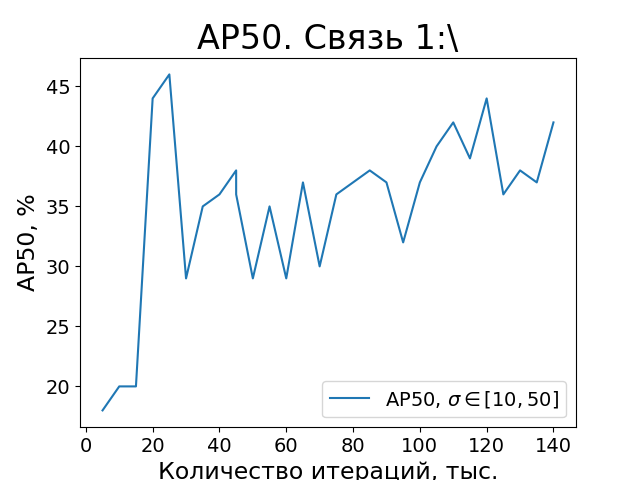
\includegraphics [scale=0.6] {my_folder/images/AP50_first}
	\caption{AP50. Первоначальный вариант обучения Faster R-CNN. Валидационная выборка. Здесь $\sigma$ -- параметр рассеяния гауссовского шума. При генерации датасета изображение зашумливалось в 2 из 3 случаях и, если зашумливалось, то параметр положения $\mu$ гауссовского шума присваивался нулю, а параметр рассеяния $\sigma$ выбирался случайным образом равномерно из диапазона $[10; 50]$}
	\label{fig:AP50_first}
\end{figure}

После того, как был получен такой результат, автор в ручном режиме просмотрел большое количество предсказанных данныхи заметил, что модель практически всегда очень точно определяет границы баундбоксов, но часто путает категории. Отсюда такие низкие показатели метрики AP.

\begin{figure}[h!] 
	\center
	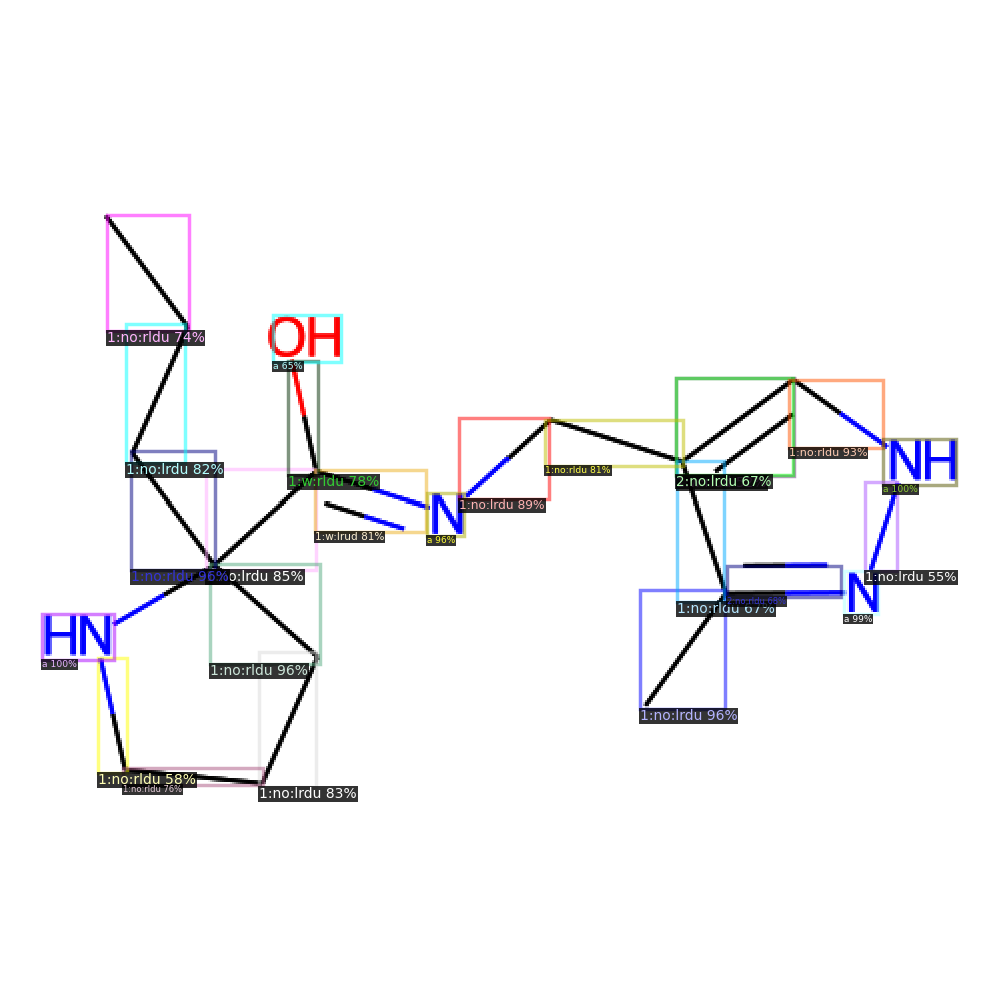
\includegraphics [scale=0.25] {my_folder/images/incorrect_faster_rcnn}
	\caption{Пример результата предсказания. Видно, что двойная связь помечена категорией \textit{1:w:lrud}, что означет сплошную клиновидную связь} 
	\label{fig:rcnn_false}
\end{figure}


\section{Итоговый конвейер моделей машинного обучения} \label{ch2:sec3}
\subsection{Изменения конвейера}
По итогам обучения первоначального варианта было замечено, что модель особенно плохо справляется с определением направления связи внутри баундбокса, в связи с чем было принято решение свести категориальный набор к следующему:

\begin{itemize}
	\item порядок связи: 1-3
	\item метка атома.
\end{itemize}

Ожидается, что уменьшение количества категорий снизит нагрузку на модуль классификации, и тем самым получится повысить качество работы object detection модели.

Для классификации направления связи используется отдельная свёрточная сеть, архитектура которой описана в разделе \ref{ch2:sec3:arch}.


\subsection{Результаты обучения итоговой object detection модели}

Приведём подробные графики всех loss функций.

\begin{figure}[h!] 
	\center
	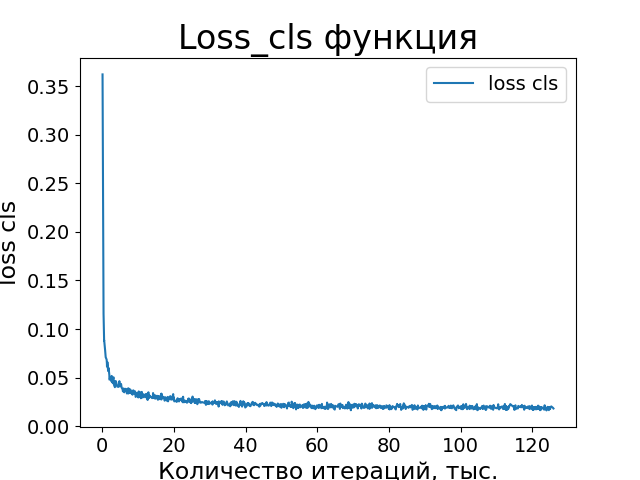
\includegraphics [scale=0.8] {my_folder/images/loss_cls_second}
	\caption{График функции loss\_cls}
	\label{fig:loss_cls}
\end{figure}

\begin{figure}[h!] 
	\center
	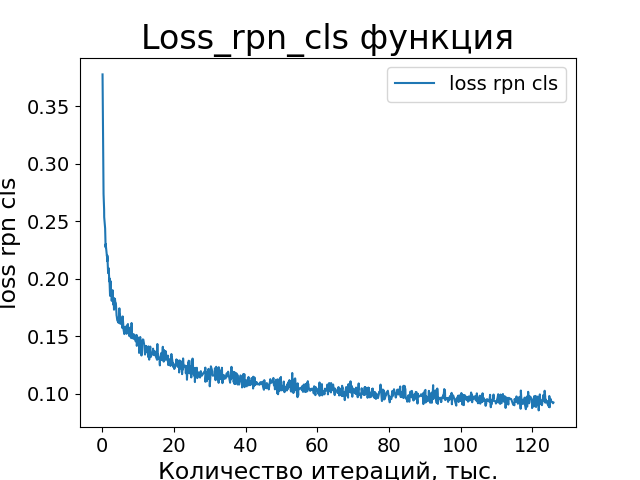
\includegraphics [scale=0.8] {my_folder/images/loss_rpn_cls_second}
	\caption{График функции loss\_rpn\_cls}
	\label{fig:loss_rpn_cls}
\end{figure}

\begin{figure}[h!] 
	\center
	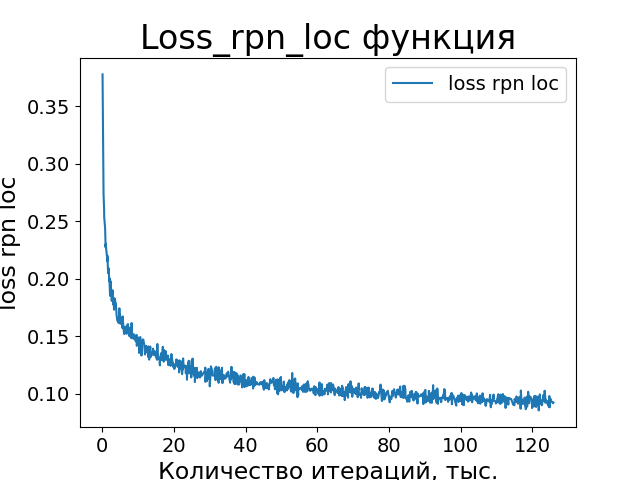
\includegraphics [scale=0.8] {my_folder/images/loss_rpn_loc_second}
	\caption{График функции loss\_rpn\_loc}
	\label{fig:loss_rpn_loc}
\end{figure}

\begin{figure}[h!] 
	\center
	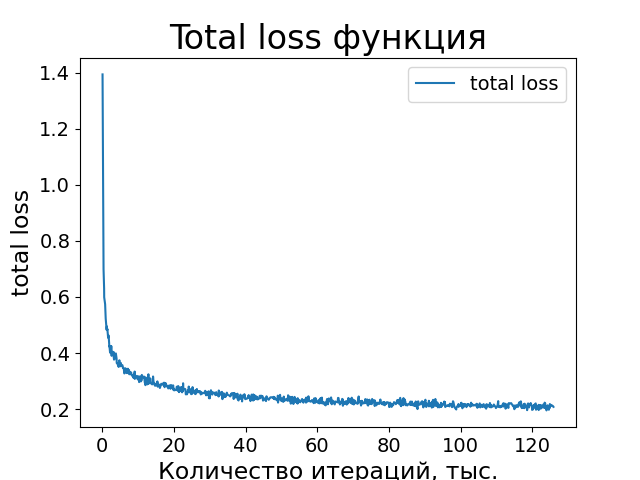
\includegraphics [scale=0.8] {my_folder/images/total_loss_second}
	\caption{График функции total\_loss}
	\label{fig:total_loss}
\end{figure}

Обучение производилось до тех пор, пока все loss-функции не выйдут на асимптоту, поскольку это является критерием окончания обучения модели.

Сопоставим графикам loss-функций графики валидационных метрик AP.

На изображении \ref{fig:AP50_second} приведено два графика AP50 для валидационной выборки. Графики соответствуют разной степени зашумленности изображения. Видно, что, во-первых, качество приблизилось к идеальному: метрика AP50 превосходит 95\% в обоих случаях, а, во-вторых, сеть устойчива к шуму: повышение амплитуды шума в два раза снизило качество обучения не более, чем на 1.5 процентных пункта.

Графики функций потерь приведены для $\sigma \in [10; 200]$.

\begin{figure}[h!] 
	\center
	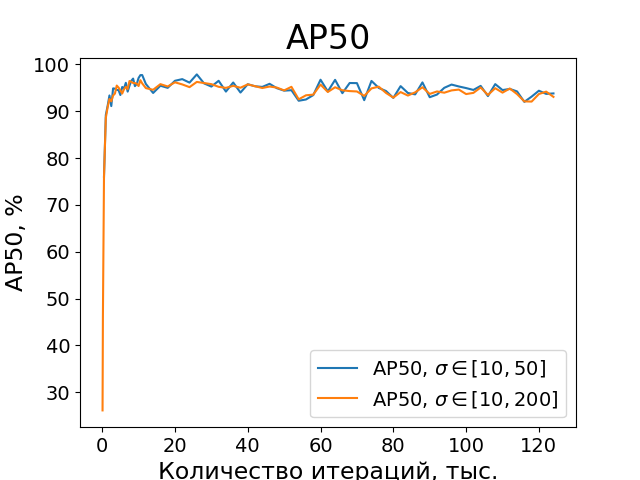
\includegraphics [scale=0.8] {my_folder/images/AP50_second}
	\caption{AP50. Итоговый вариант обучения Faster R-CNN. Валидационная выборка. Приведено два графика для разных степеней зашумленности изображения: $\sigma \in [10; 50], \; \sigma \in [10; 200]$}
	\label{fig:AP50_second}
\end{figure}

Стоит обратить внимание на то, что несмотря на достаточно медленную сходимость сети (выход на асимптоту по всем функциям потерь происходит примерно к 80-100 тысячам итераций), метрики качества выходят на асимптоту гораздо раньше.

\subsection{Архитектура вспомогательных нейронных сетей. Генерация данных} \label{ch2:sec3:arch}

Для классификации направлений связи и меток атомов были обучены две свёрточные нейронные сети с одинаковой архитектурой:
использовались два свёрточных слоя, flatten, dropout и dense слои.

\begin{figure}[h!] 
	\center
	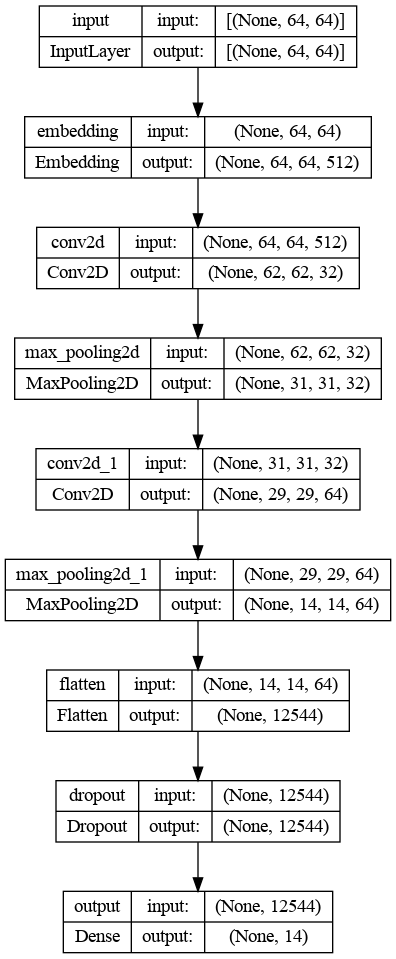
\includegraphics [scale=0.3] {my_folder/images/model_bond}
	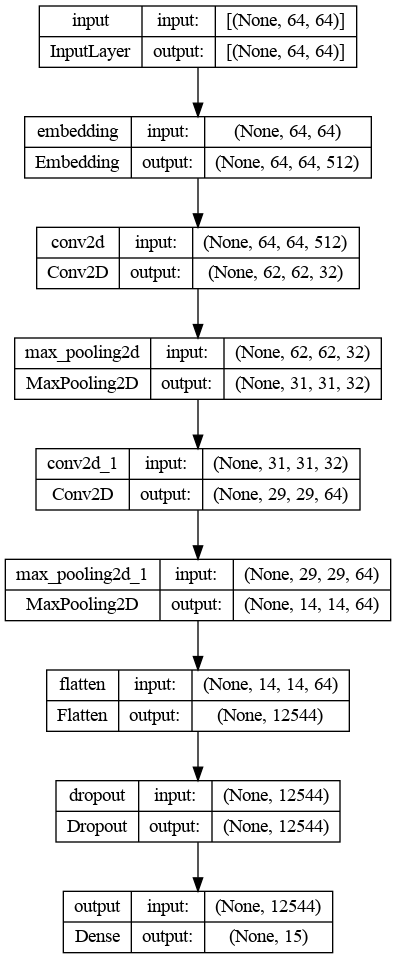
\includegraphics [scale=0.3] {my_folder/images/model_atom}
	\caption{Архитектура CNN для распознавания связей (слева) и меток атомов (справа)}
	\label{fig:AP50_modelbondatom}
\end{figure}

Для генерации обучающих данных использовались ранее сгенерированные для обучения object detection модели изображения. Был сформирован идеально сбалансированный датасет: на каждую категорию сгенерировано по 1000 изображений.

\subsection{Результаты обучения классификаторов}

Обучение производилось в обоих случаях на 50 эпохах, 1500 экземпляров на категорию.

Метрики классификатора категорий связи смотрите в таблице 2.1.

\begin{table}[htbp]% Пример оформления таблицы
	\centering
	\label{tab:bondquality}		
		\begin{tabular}{|c|c|c|}
			\hline
			$F_{1_{\min}}$ & $F_{1_{\max}}$ & $F_{1_{avg}}$ \\
			\hline
			0.97 & 0.99 & 0.98 \\
			\hline
		\end{tabular}
	\caption{Качество обучения классификатора связей}
\end{table}

\begin{figure}[h!] 
	\center
	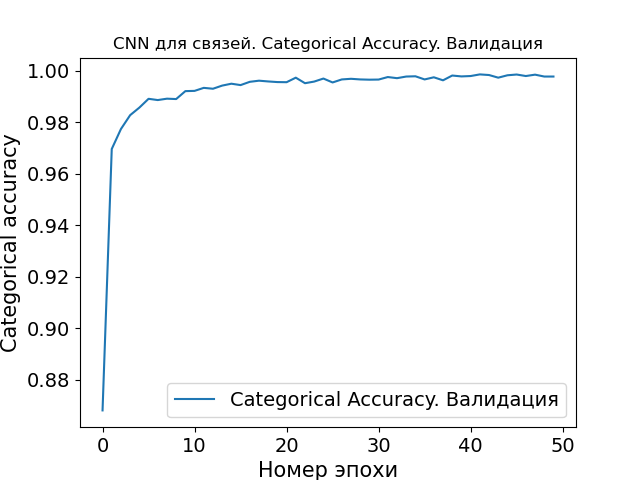
\includegraphics [scale=0.8] {my_folder/images/bonddir_accuracy}
	\caption{График зависимости метрики categorical accuracy от номера эпохи для классификатора категорий связей}
	\label{fig:AP50_bonddir_accuracy}
\end{figure}

\begin{figure}[h!] 
	\center
	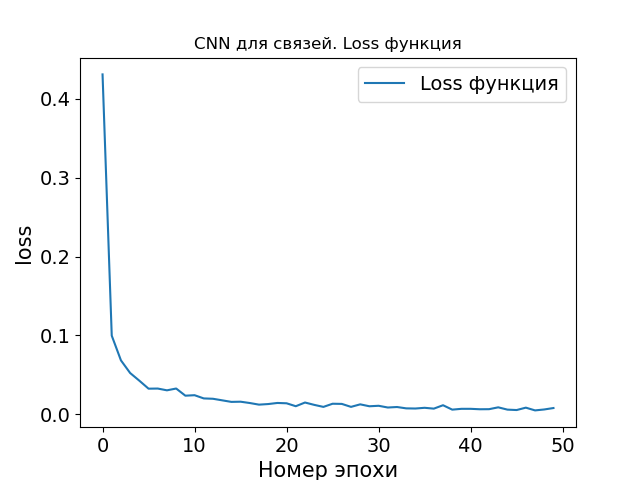
\includegraphics [scale=0.8] {my_folder/images/bonddir_loss}
	\caption{График зависимости функции потерь от номера эпохи для классификатора категорий связей}
	\label{fig:AP50_bonddir_loss}
\end{figure}

Метрики классификатора меток атомов смотрите в таблице 2.2.

\begin{table}[htbp]% Пример оформления таблицы
	\centering
	\label{tab:atomquality}		
	\begin{tabular}{|c|c|c|}
		\hline
		$F_{1_{\min}}$ & $F_{1_{\max}}$ & $F_{1_{avg}}$ \\
		\hline
		0.96 & 0.98 & 0.9\ \\
		\hline
	\end{tabular}
	\caption{Качество обучения классификатора меток атомов}
\end{table}

\begin{figure}[h!] 
	\center
	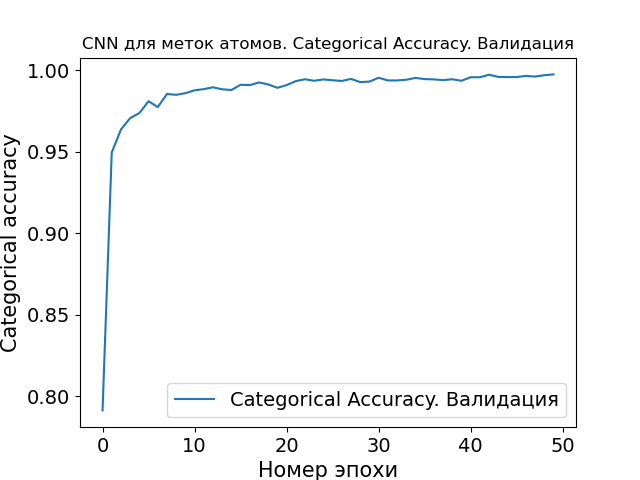
\includegraphics [scale=0.8] {my_folder/images/atom_accuracy}
	\caption{График зависимости метрики categorical accuracy от номера эпохи для классификатора меток атомов}
	\label{fig:AP50_atom_accuracy}
\end{figure}

\begin{figure}[h!] 
	\center
	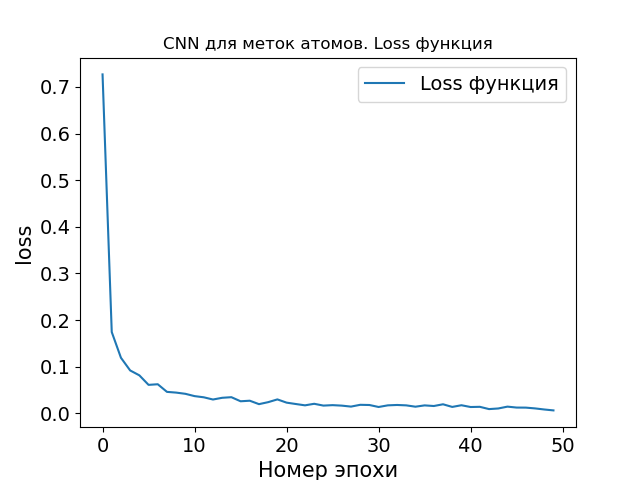
\includegraphics [scale=0.8] {my_folder/images/atom_loss}
	\caption{График зависимости функции потерь от номера эпохи для классификатора меток атомов}
	\label{fig:AP50_atom_loss}
\end{figure}


%\input{my_folder/tex/rules-list-of-environments} % список некоторых окружений
%\input{my_folder/tex/tab-toy-context-minipage} % пример подключения minipage
%\input{my_folder/tex/fig-spbpu-new-bld-autumn-minipage} % пример подключения minipage
%\input{my_folder/tex/rules-theorem-like-expressions} 
%\input{my_folder/tex/theorem-example} %пример оформления теоремы
%\input{my_folder/tex/definition-example} %пример оформления определения
%\input{my_folder/tex/eq-equation-multilined} % пример оформления одиночной формулы в несколько строк
%\input{my_folder/tex/fig-spbpu-sc-four-in-one} % пример подключения 4х иллюстраций в одном рисунке

\FloatBarrier % заставить рисунки и другие подвижные (float) элементы остановиться
\NewPage

